\lstset{language=json}
\chapter{Routen der REST-API}
Im folgenden Kapitel werden die Routen beschrieben, die Shulker-Connect als REST-API bereitstellt.

\subsection{/api/Credentials}
\begin{lstlisting}
GET /api/Credentials
\end{lstlisting}

\textbf{Beschreibung:} \\
Gibt eine Liste aller Pins zurück.

\textbf{Rückgabe:} \\
Liste aller Pins im JSON-Format.

\begin{figure}[H]
    \begin{center}
        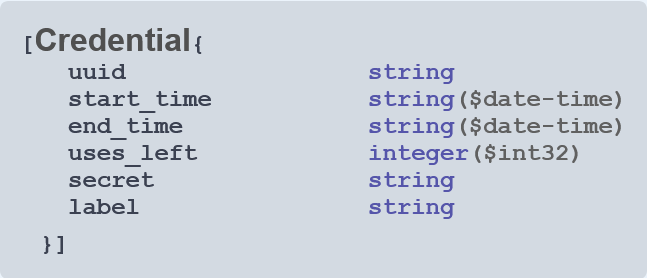
\includegraphics[width=.5\textwidth]{images/connect/routes/Credentials.png}
        \caption{Rückgabe der Route}
    \end{center}
\end{figure}

\subsubsection{Parameter}
\textit{[Erforderlich]} \textbf{session} \\
Typ: \textbf{string} \\
Beschreibung: Session-String zur Authentifikation.

\subsubsection{Beispiel}
\begin{lstlisting}
GET    /api/Credentials?session=duHSYvYpBMzaekLGruTLosFECRTIKweC
\end{lstlisting}
\textbf{Beispielhafte Antwort} \\
\begin{lstlisting}
[
    {
        "uuid": "58813b36-d3d9-4255-b212-6376e0b9fe17",
        "start_time": "2022-03-19T16:40:34.098Z",
        "end_time": "9999-01-01T15:00:00Z",
        "uses_left": -1,
        "secret": null,
        "label": "Mama"
      }
]
\end{lstlisting}







\subsection{/api/Credentials/createPin}
\begin{lstlisting}
POST /api/Credentials/createPin
\end{lstlisting}

\textbf{Beschreibung:} \\
Erstellt einen neuen Pin.

\textbf{Rückgabe:} \\
Bei Erfolg: \textit{HTTP 200 Success} \\
Bei ungültiger Anfrage: \textit{HTTP 400 Bad Request}

\subsubsection{Parameter}
\textit{[Erforderlich]} \textbf{session} \\
Typ: \textbf{string} \\
Beschreibung: Session-String zur Authentifikation. \\


\textit{[Erforderlich]} \textbf{Credential} \\
Typ: \textbf{Credential} \\
Beschreibung: Das zu erstellende Credential. \\


\subsubsection{Beispiel}
\begin{lstlisting}
POST    /api/Credentials/createPin
{
  "uuid": "58813b36-d3d9-4255-b212-6376e0b9fe17",
  "start_time": "2022-03-19T16:40:34.098Z",
  "end_time": "9999-01-01T15:00:00.000Z",
  "uses_left": -1,
  "secret": "14205735",
  "label": "Mama"
}
\end{lstlisting}
\textbf{Beispielhafte Antwort} \\
\textit{HTTP 200 Success}




\subsection{/api/Credentials/deletePin/{uuid}}
\begin{lstlisting}
DELETE /api/Credentials/deletePin/{uuid}
\end{lstlisting}

\textbf{Beschreibung:} \\
Löscht einen existierenden Pin.

\subsubsection{Parameter}
\textit{[Erforderlich]} \textbf{session} \\
Typ: \textbf{string} \\
Beschreibung: Session-String zur Authentifikation. \\

\textit{[Erforderlich]} \textbf{uuid} \\
Typ: \textbf{string} \\
Beschreibung: UUID des zu löschenden Pins.

\subsubsection{Beispiel}
\begin{lstlisting}
POST    /api/Credentials/deletePin/{uuid}
{
  "session": "BzPwGtFJgCeXdOxxtiWSWott4u7AxaNk",
  "uuid": "58813b36-d3d9-4255-b212-6376e0b9fe17"
}
\end{lstlisting}
\textbf{Beispielhafte Antwort} \\
\textit{HTTP 200 Success}





\subsection{/api/Lock/isLocked}
\begin{lstlisting}
GET /api/Lock/isLocked
\end{lstlisting}

\textbf{Beschreibung:} \\
Gibt zurück, ob das Türschloss gerade geöffnet oder geschlossen ist. 

\textbf{Rückgabe:} \\
\textit{boolean}: true/false

\subsubsection{Parameter}
\textit{[Erforderlich]} \textbf{session} \\
Typ: \textbf{string} \\
Beschreibung: Session-String zur Authentifikation. 

\subsubsection{Beispiel}
\begin{lstlisting}
GET    /api/Lock/isLocked

\end{lstlisting}
\textbf{Beispielhafte Antwort} \\
\textit{true}





\subsection{/api/Lock/setLockState}
\begin{lstlisting}
POST /api/Lock/setLockState
\end{lstlisting}

\textbf{Beschreibung:} \\
Öffnet bzw. schließt das Türschloss 

\subsubsection{Parameter}
\textit{[Erforderlich]} \textbf{session} \\
Typ: \textbf{string} \\
Beschreibung: Session-String zur Authentifikation.\\

\textit{[Erforderlich]} \textbf{closed} \\
Typ: \textbf{boolean} \\
Soll das Schloss geschlossen sein.

\subsubsection{Beispiel}
\begin{lstlisting}
POST    /api/Lock/setLockState
{
    "closed": "false"
}
\end{lstlisting}
Öffnet das Türschloss

\textbf{Beispielhafte Antwort} \\
\textit{HTTP 200 Success}





\subsection{/api/Session/getToken/{secret}}
\begin{lstlisting}
GET /api/Session/getToken/{secret}
\end{lstlisting}

\textbf{Beschreibung:} \\
Generiert eine neue Session für die Authentifikation.

\subsubsection{Parameter}
\textit{[Erforderlich]} \textbf{session} \\
Typ: \textbf{string} \\
Beschreibung: Session-String zur Authentifikation.\\

\textit{[Erforderlich]} \textbf{secret} \\
Typ: \textbf{string} \\
Das Master-Passwort des Türschlosses.

\subsubsection{Beispiel}
\begin{lstlisting}
GET    /api/Session/getToken/master123
\end{lstlisting}

\textbf{Beispielhafte Antwort} \\
\textit{AJr4O2VE8bT3DeCW5rG4yyB1Esy1vXJY}





\subsection{/api/Status}
\begin{lstlisting}
GET /api/Status
\end{lstlisting}

\textbf{Beschreibung:} \\
Kann verwendet werden, um zu überprüfen, ob die Kommunikation zum API-Server funktioniert.

\textbf{Rückgabe:} \\
\textit{HTTP 200 Success}

\subsubsection{Beispiel}
\begin{lstlisting}
GET    /api/Status
\end{lstlisting}

\textbf{Beispielhafte Antwort} \\
\textit{HTTP 200 Success}


\chapter{Routen der Interprozesskommunikation}
toDO